% Made up for the tikra benchmark.
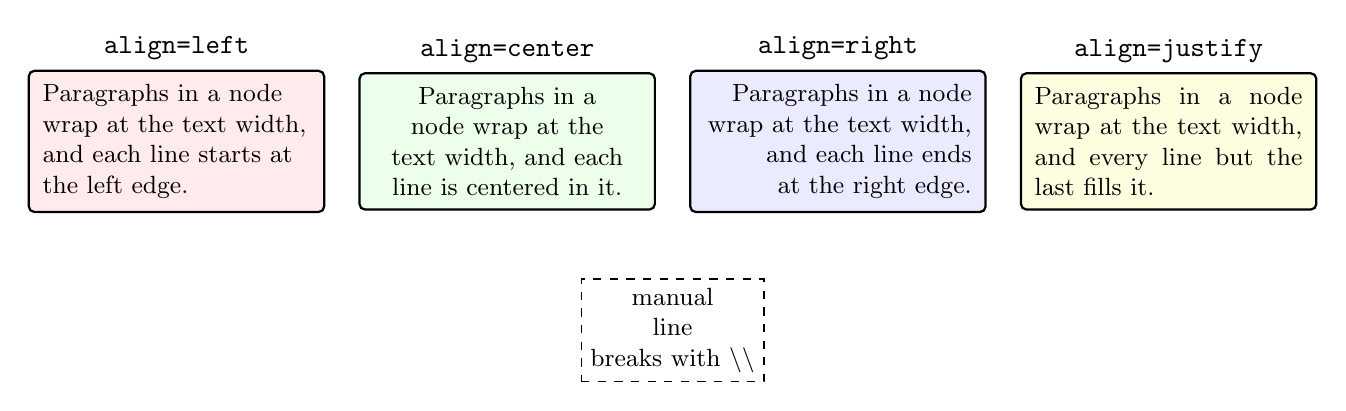
\begin{tikzpicture}[box/.style={draw, thick, rounded corners=2pt, text width=3.4cm, inner sep=5pt, font=\small}]
  \node[box, align=left, fill=red!8, label=above:\texttt{align=left}] at (0,0)
    {Paragraphs in a node wrap at the text width, and each line starts at the left edge.};
  \node[box, align=center, fill=green!8, label=above:\texttt{align=center}] at (4.2,0)
    {Paragraphs in a node wrap at the text width, and each line is centered in it.};
  \node[box, align=right, fill=blue!8, label=above:\texttt{align=right}] at (8.4,0)
    {Paragraphs in a node wrap at the text width, and each line ends at the right edge.};
  \node[box, align=justify, fill=yellow!12, label=above:\texttt{align=justify}] at (12.6,0)
    {Paragraphs in a node wrap at the text width, and every line but the last fills it.};
  \node[draw, dashed, align=center, font=\small] at (6.3,-2.4) {manual\\line\\breaks with \texttt{\textbackslash\textbackslash}};
\end{tikzpicture}
